\documentclass[11pt,a4paper]{article}
\usepackage[utf8]{inputenc}
\usepackage[T1]{fontenc}
\usepackage[spanish,es-noshorthands]{babel}
\usepackage[margin=2.2cm]{geometry}
\usepackage{amsmath,amssymb,bm}
\usepackage{graphicx}
\usepackage{booktabs}
\usepackage{xcolor}
\usepackage{enumitem}
\usepackage[colorlinks=true,linkcolor=blue!50!black,urlcolor=blue!50!black]{hyperref}
\graphicspath{{./}{../}}
\setlength{\parskip}{4pt}
\setlength{\parindent}{0pt}
\newcommand{\atan}{\operatorname{atan2}}
\title{Cinemática de la pata del Segway: resumen de los cálculos\\
\large Mecanismo de cuatro barras \(A\,B\,C\,D\) con acoplador rígido \(C\,D\,P\)}
\author{Proyecto Segway con patas -- Robótica II, UNCUYO}
\date{\today}

\begin{document}
\maketitle

\section{Geometría y notación}

Todo se mide en el plano lateral del robot, con origen en \(A\) (eje del servo), \(x\) positivo hacia
atrás e \(y\) positivo hacia arriba. Los segmentos se nombran por sus extremos; los ángulos son
antihorarios desde \(+x\).

\begin{center}

\includegraphics[width=0.98\textwidth]{geometria_robot.png}
\end{center}

\begin{center}
\small
\begin{tabular}{llcl}
\toprule
Símbolo & Qué es & Valor CAD & Pieza \\
\midrule
\(AB\) & bancada: distancia entre los pivotes \(A\) y \(B\) de la cabina & 100 mm & \texttt{cabeza\_v31} \\
\(\beta\) & ángulo de \(A\!\to\!B\) desde \(+x\) & \(45^\circ\) & \texttt{cabeza\_v31} \\
\(AD\) & manivela (la mueve el servo) & 140 mm & \texttt{eslabon\_AD} \\
\(BC\) & balancín & 135 mm & \texttt{eslabon\_BC} \\
\(CD\) & acoplador, tramo \(C\)--\(D\) & 51 mm & \texttt{eslabon\_CDP} \\
\(DP\) & acoplador, tramo \(D\)--\(P\) (hasta el eje de rueda) & 140 mm & \texttt{eslabon\_CDP} \\
\(\delta\) & ángulo del acoplador en \(D\), de \(D\!\to\!C\) a \(D\!\to\!P\) & \(164^\circ\) (plano: \(16^\circ\)) & \texttt{eslabon\_CDP} \\
\(\theta\) & ángulo del servo: dirección de \(A\!\to\!D\) desde \(+x\) & \(320^\circ\) a \(350^\circ\) & servo en \(A\) \\
\(R_w\) & radio de rueda & 33 mm & \texttt{wheel} \\
\bottomrule
\end{tabular}
\end{center}

Variables intermedias que aparecen en la deducción: \(BD\) (diagonal), \(\alpha_{DB}\) (dirección de
\(D\!\to\!B\)), \(\gamma\) (ángulo en \(D\) del triángulo \(BDC\)), \(\theta_{DC}\), \(\theta_{DP}\)
(direcciones de \(D\!\to\!C\) y \(D\!\to\!P\)), \(\theta_{BC}\) (dirección del balancín) y \(\mu\)
(ángulo de transmisión en \(C\)). La entrada es \(\theta\); la salida que interesa es la posición del
eje de rueda \(P=(x_P,\,y_P)\).

\section{Cinemática directa: de \(\theta\) a \(P\)}

\begin{center}
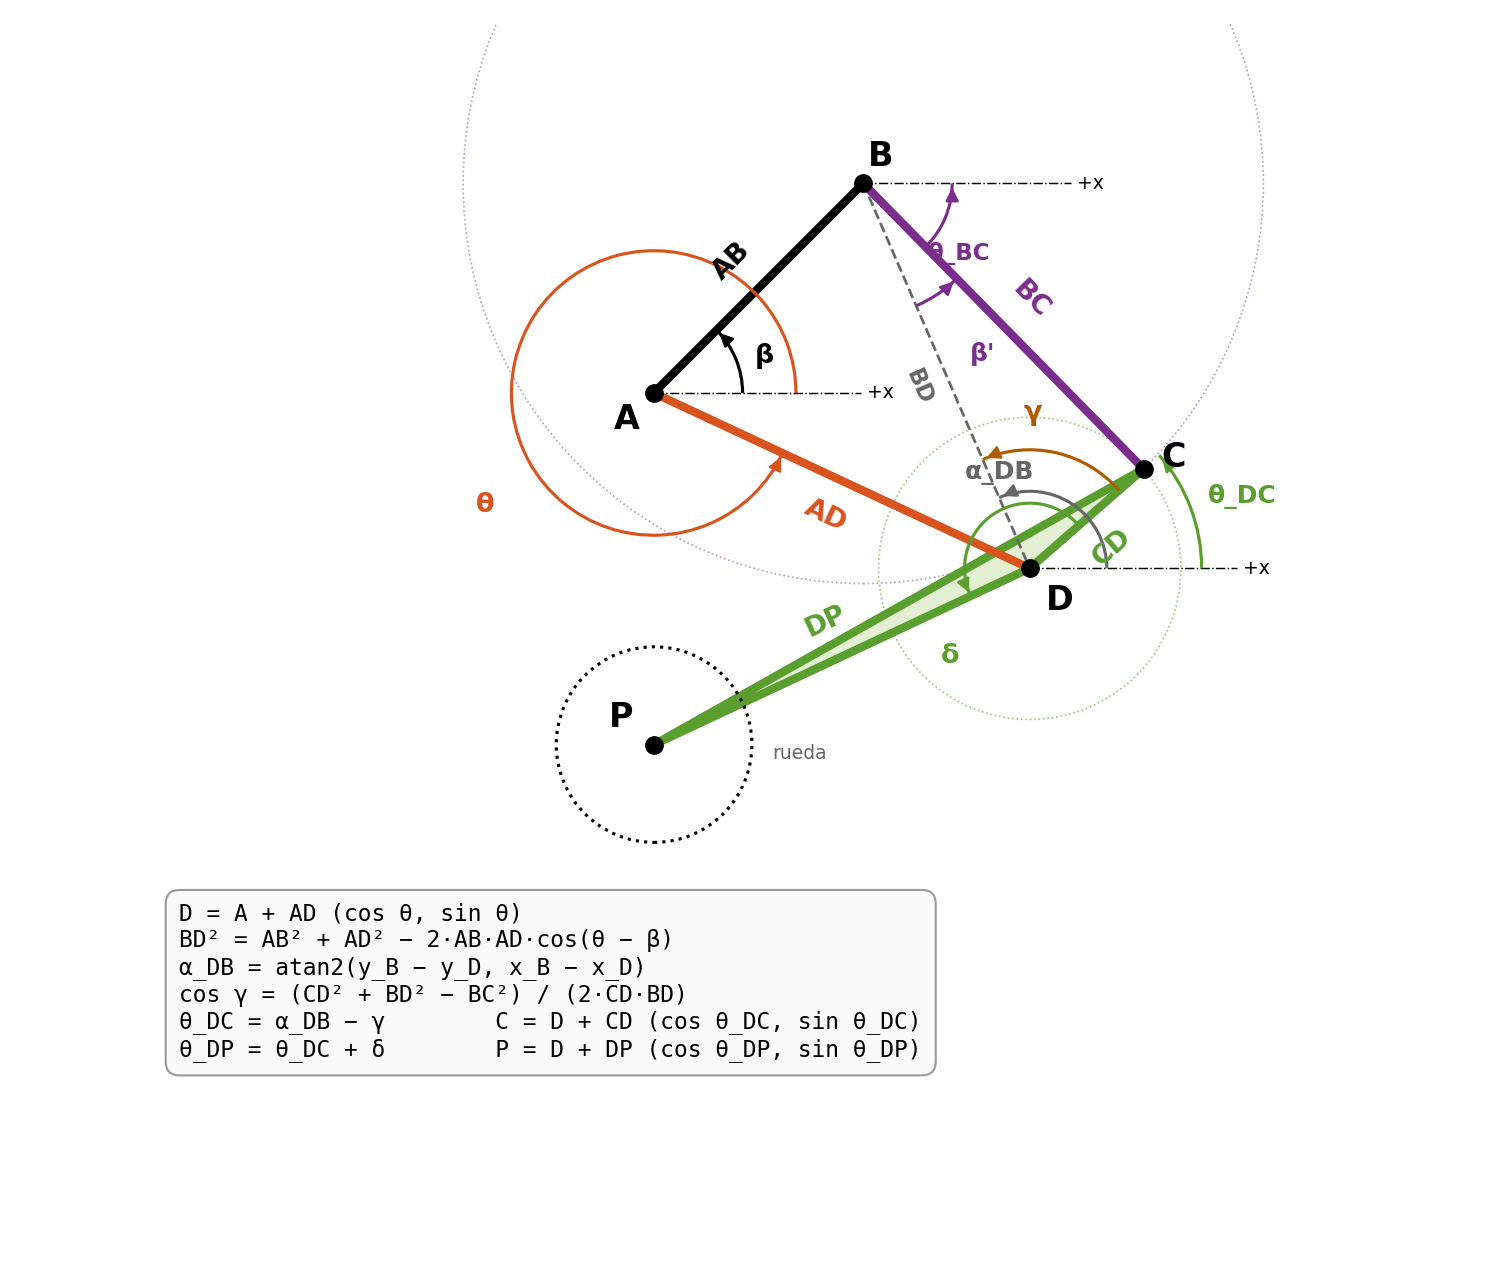
\includegraphics[width=0.8\textwidth]{fig_cinematica_directa.png}
\end{center}

\textbf{Datos fijos.} \(A=(0,0)\) y \(B=(x_B,y_B)=(AB\cos\beta,\;AB\sin\beta)\).

\textbf{Paso 1: la manivela.} El servo fija la dirección de \(A\!\to\!D\):
\begin{equation}
D=(x_D,y_D)=\bigl(AD\cos\theta,\;AD\sin\theta\bigr).
\end{equation}

\textbf{Paso 2: la diagonal \(BD\).} Es el lado del triángulo \(ABD\) opuesto al ángulo
\(\theta-\beta\) en \(A\); por la ley del coseno,
\begin{equation}
BD^2=AB^2+AD^2-2\,AB\,AD\cos(\theta-\beta),
\qquad
\alpha_{DB}=\atan\!\bigl(y_B-y_D,\;x_B-x_D\bigr).
\label{eq:BD}
\end{equation}

\textbf{Paso 3: el ángulo \(\gamma\) en \(D\).} En el triángulo \(BDC\) se conocen los tres lados
(\(BD\), \(CD\), \(BC\)); la ley del coseno da el ángulo en \(D\), entre \(D\!\to\!B\) y \(D\!\to\!C\):
\begin{equation}
\cos\gamma=\frac{CD^2+BD^2-BC^2}{2\,CD\,BD}.
\label{eq:gamma}
\end{equation}
El mecanismo cierra sólo si \(|BC-CD|\le BD\le BC+CD\) (equivale a \(|\cos\gamma|\le1\)). Es la
misma cuenta que intersecar la circunferencia de centro \(B\) y radio \(BC\) con la de centro \(D\) y
radio \(CD\).

\textbf{Paso 4: el punto \(C\).} Las dos intersecciones son \(\theta_{DC}=\alpha_{DB}\pm\gamma\). El CAD
está armado con \(C\) a la derecha de \(D\!\to\!B\) (\(C\) queda atrás y arriba de \(D\)), que es el
signo menos:
\begin{equation}
\theta_{DC}=\alpha_{DB}-\gamma,\qquad
C=\bigl(x_D+CD\cos\theta_{DC},\;y_D+CD\sin\theta_{DC}\bigr).
\end{equation}
La otra rama (\(\alpha_{DB}+\gamma\)) es la configuración cruzada del cuatro barras y no se usa.
Con el mismo criterio, visto desde \(B\): \(\theta_{BC}=\alpha_{BD}+\beta'\), con
\(\cos\beta'=(BC^2+BD^2-CD^2)/(2\,BC\,BD)\) y \(\alpha_{BD}=\alpha_{DB}+180^\circ\).

\textbf{Paso 5: el punto \(P\).} El acoplador es rígido: la dirección de \(D\!\to\!P\) está a \(\delta\)
de la de \(D\!\to\!C\):
\begin{equation}
\theta_{DP}=\theta_{DC}+\delta,\qquad
P=\bigl(x_D+DP\cos\theta_{DP},\;y_D+DP\sin\theta_{DP}\bigr).
\end{equation}

\subsection*{Ecuación final}

Reemplazando los pasos anteriores, la posición del eje de rueda en función del ángulo del servo es
\begin{equation}
\boxed{\;
\begin{aligned}
x_P(\theta)&=AD\cos\theta+DP\cos\bigl(\alpha_{DB}(\theta)-\gamma(\theta)+\delta\bigr),\\[2pt]
y_P(\theta)&=AD\sin\theta+DP\sin\bigl(\alpha_{DB}(\theta)-\gamma(\theta)+\delta\bigr),
\end{aligned}\;}
\label{eq:final}
\end{equation}
con
\begin{gather}
BD(\theta)=\sqrt{AB^2+AD^2-2\,AB\,AD\cos(\theta-\beta)},\qquad
\gamma(\theta)=\arccos\frac{CD^2+BD(\theta)^2-BC^2}{2\,CD\,BD(\theta)},\\[2pt]
\alpha_{DB}(\theta)=\atan\!\bigl(AB\sin\beta-AD\sin\theta,\;AB\cos\beta-AD\cos\theta\bigr).
\end{gather}
La altura del eje del servo sobre el piso es \(z_A=R_w-y_P(\theta)\), y la altura del eje de rueda
sobre el piso es \(R_w\).

\section{Cinemática inversa: de una altura a \(\theta\)}

Dada la altura deseada \(y_P^{*}\) hay que resolver \(y_P(\theta)=y_P^{*}\). La ecuación es
trascendente en \(\theta\) (aparecen \(\theta\) dentro de \(\arccos\) y de \(\atan\)) y no tiene
solución cerrada útil. En el recorrido del servo \(y_P(\theta)\) es monótona creciente (tabla de la
sección~\ref{sec:num}), así que la solución es única y se obtiene por bisección o con una tabla
\(\theta\leftrightarrow y_P\) interpolada. Eso hace \texttt{cinematica\_inversa.m}.

\section{Verificación numérica}\label{sec:num}

Con los valores del CAD, ecuación~\eqref{eq:final} evaluada en tres puntos del recorrido (mm y grados):

\begin{center}
\small
\begin{tabular}{ccccccccc}
\toprule
\(\theta\) & \(BD\) & \(\alpha_{DB}\) & \(\gamma\) & \(\theta_{DC}\) & \(D\) & \(C\) & \(P\) & \(z_A\) \\
\midrule
320 & 164.8 & 102.8 & 46.7 & 56.1 & (107.3, \(-90.0\)) & (135.7, \(-47.6\)) & (0.2, \(-180.3\)) & 213.2 \\
335 & 141.5 & 113.4 & 72.3 & 41.1 & (126.9, \(-59.2\)) & (165.3, \(-25.6\)) & (0.1, \(-118.6\)) & 151.6 \\
350 & 116.4 & 125.3 & 100.1 & 25.1 & (137.9, \(-24.3\)) & (184.0, \(-2.6\)) & (\(-0.3\), \(-46.6\)) & 79.5 \\
\bottomrule
\end{tabular}
\end{center}

\begin{itemize}[nosep]
\item Las longitudes \(|AD|,|BC|,|CD|,|DP|\) recalculadas desde los puntos coinciden con las cotas con
error menor que \(10^{-12}\) mm, y la ecuación~\eqref{eq:final} coincide con la construcción por
intersección de circunferencias del script del grupo con error menor que \(10^{-12}\) mm.
\item En todo el recorrido \(BD\in[116,\,165]\) mm, dentro de \([\,|BC-CD|,\,BC+CD\,]=[84,\,186]\) mm:
el mecanismo cierra siempre. El ángulo de transmisión en \(C\) va de \(63^\circ\) a \(58^\circ\)
(mayor que \(40^\circ\): sin riesgo de trabarse).
\item Carrera del eje de rueda entre \(320^\circ\) y \(350^\circ\): \(133.7\) mm vertical, con un desvío
horizontal de sólo \(0.6\) mm. Con \(AB=100\) mm a \(45^\circ\) el mecanismo hace la línea recta
para la que fue diseñado (con la bancada anterior, de 80 mm a \(47.5^\circ\), el desvío era de 9 mm).
\end{itemize}

\section{Revisión de la cinemática que estaba en \texttt{modelado/cinematica}}

\begin{enumerate}[nosep]
\item \textbf{Las ecuaciones estaban bien.} Las hojas manuscritas y \texttt{verificar\_cinematica\_4barras.m}
hacen exactamente los pasos 1 a 5 (ley del coseno + intersección de circunferencias). Sólo se
reordenaron con un nombre por segmento (\(AB\), \(AD\), \(BC\), \(CD\), \(DP\)) y las cotas en un único
archivo, \texttt{parametros\_geometria.m}.
\item \textbf{Bancada.} En las hojas \(B=(L,0)\); en el CAD \(B=AB(\cos\beta,\sin\beta)\) con
\(\beta=45^\circ\). El script ya usaba \(45^\circ\); las hojas no.
\item \textbf{Signo de la rama.} Las hojas dejan \(\theta_{BC}=\alpha_{BD}\pm\beta'\) sin decidir. Para
la configuración del CAD es \(\theta_{DC}=\alpha_{DB}-\gamma\) (equivalentemente
\(\theta_{BC}=\alpha_{BD}+\beta'\)). La otra rama lleva \(P\) a \((204,\,-192)\) mm con
\(\theta=320^\circ\): la pata cruzada.
\item \textbf{Ángulo \(\delta\).} Las hojas escriben \(P=D-DP\,(\cos(\theta_{DC}-16^\circ),\,\sin(\theta_{DC}-16^\circ))\);
es lo mismo que \(\theta_{DP}=\theta_{DC}+164^\circ\) (el signo menos es el giro de \(180^\circ\)).
Conviene usar una sola forma: \(\delta=164^\circ\) antihorario desde \(D\!\to\!C\).
\item \textbf{Nombres.} En las hojas aparecen \(L_{CP}=1{,}4L\) y \(L_{DP}\) para el mismo tramo, y
\(L_{DC}\)/\(L_{CD}\); quedó \(DP\) y \(CD\).
\item \textbf{Unidades.} El script trabajaba en cm con \(L=10\); ahora todo está en mm con las cotas
reales del CAD y el radio de rueda de 33 mm (antes 37,5 mm).
\end{enumerate}

\subsection*{Archivos}
\begin{itemize}[nosep]
\item \texttt{modelado/geometria\_robot.png} (y \texttt{.py}): figura de la geometría con nombres y valores.
\item \texttt{modelado/cinematica/parametros\_geometria.m}: las cotas (única fuente).
\item \texttt{modelado/cinematica/cinematica\_directa.m}: ecuaciones \eqref{eq:BD} a \eqref{eq:final}.
\item \texttt{modelado/cinematica/cinematica\_inversa.m}: \(\theta\) para una altura dada (bisección).
\item \texttt{modelado/cinematica/verificar\_cinematica\_4barras.m}: la animación del grupo, usando lo anterior.
\end{itemize}

\end{document}
